\documentclass[12pt]{article}
%\documentclass[12pt,a4paper]{report}
\usepackage[a4paper,margin=1in]{geometry}
\usepackage{graphicx}
\usepackage{subcaption}
\usepackage{float}
\usepackage{booktabs}
\usepackage{listings}


\lstset{
    language=Python,
    basicstyle=\ttfamily\small,
    keywordstyle=\color{blue}\bfseries,
    commentstyle=\color{green!60!black},
    stringstyle=\color{red},
    numbers=left,
    numberstyle=\tiny,
    stepnumber=1,
    numbersep=8pt,
    showstringspaces=false,
    frame=single,
    breaklines=true,
    tabsize=4,
    captionpos=b
}
\usepackage{xcolor}
\usepackage{amsmath}
\usepackage{hyperref}
\hypersetup{
    colorlinks=true,
    linkcolor=blue,
    urlcolor=blue,
    citecolor=black
}
\usepackage{enumitem}
\usepackage{tikz}
\usetikzlibrary{positioning,arrows.meta}
\usetikzlibrary{shapes.geometric, arrows.meta, positioning}
\usepackage{fancyhdr}
\fancypagestyle{introstyle}{\fancyhf{}
    \fancyfoot[L]{%
        \footnotesize Internship Report\\
        Lakshya, NISER Bhubaneswar}
    \fancyfoot[R]{\thepage}
    \renewcommand{\headrulewidth}{0pt}
    \renewcommand{\footrulewidth}{0pt}}
\setcounter{secnumdepth}{4}
\setcounter{tocdepth}{4}
\begin{document}
\begin{center}
{\LARGE \textbf{NISER Summer Internship Report}}\\
\vspace{0.4cm}
{\Large\textbf{On}}\\
\vspace{0.4 cm}
{\Large \textbf{Vision-Based Autonomous Drone System}}\\
\vspace{0.8 cm}

\includegraphics[width=0.3\textwidth]{/home/lakshya/Downloads/logo.png}\\
\vspace{0.8cm}
{\large Lakshya}\\
\vspace{0.8 cm}
{\large Integrated M.sc 2025}\\
\vspace{0.8 cm}
{\large {NATIONAL INSTITUTE OF SCIENCE EDUCATION AND RESEARCH(NISER)}}\\
\vspace{0.8 cm}
{\large Project Guid: Prof.Subhankar Mishra}\\
\vspace{0.8 cm}
%{\large Project Mentor: Mr.Jyothish Kumar J}\\
%\vspace{0.8 cm}
{\large Tenure: 17th may - 30th june}\\
\vspace{0.8 cm}
{\large Submission Date: \today}
\end{center}
%\maketitle
\newpage
\section*{Acknowledgement}
\thispagestyle{introstyle}
\large{I would like to express my sincere gratitude to \textbf{Prof. Subhankar Mishra} for their invaluable guidance, continuous support, and encouragement throughout this project. I would also like to extend my special thanks to\textbf{ Mr.Jyothish Kumar J} for their constant motivation, insightful suggestions, and generous assistance, which greatly contributed to the successful completion of this work.I am thankful to the \textbf{RoboTech Club NISER} for providing the opportunity, resources, and a collaborative environment to carry out this project. I also express my sincere appreciation to the \textbf{National Institute of Science Education and Research (NISER), Bhubaneswar}, for providing an excellent academic environment and the facilities necessary for this work.Finally, I am grateful to everyone who contributed directly or indirectly to the successful completion of this project.
}

\newpage
\tableofcontents
\thispagestyle{introstyle}
\newpage
\section{Introduction}
\thispagestyle{introstyle}
\large{Unmanned Aerial Vehicles \textbf{(UAVs)}, commonly known as drones, have become increasingly important in applications such as surveillance, infrastructure inspection, environmental monitoring, agriculture, mapping, and autonomous navigation. Recent advances in computer vision and embedded systems have enabled drones to perform intelligent tasks with minimal human intervention.\\
The primary objective of this internship was to study and develop the fundamental components required for a vision-based autonomous drone system. The work involved establishing communication between a \textbf{Raspberry Pi} and a \textbf{Pixhawk flight controller} using the \textbf{MAVLink protocol}, configuring and calibrating the drone platform, performing camera calibration, detecting ArUco markers using OpenCV, estimating marker pose and distance, and developing a vision-based tracking framework.
The project aims to provide a foundation for future autonomous functionalities such as object tracking, precision landing, docking, and autonomous navigation. By integrating computer vision with flight control systems, the developed framework contributes towards building reliable and intelligent UAV applications.

\newpage
\section{Overview and structure}
\thispagestyle{introstyle}
This report presents the work carried out during the internship on the development of a vision-based tracking system and its transition towards an autonomous drone platform. The project combines computer vision techniques with UAV technology to establish the foundation for applications such as object tracking, precision landing, docking, surveying, and autonomous navigation.The report is organized into several chapters, each describing a specific stage of the project. Following the introduction, the project objectives are presented, outlining the primary goals and intended applications of the developed system. The hardware and software tools used throughout the project are then described.Subsequent chapters discuss the evolution of the project and the architecture of the vision tracking system, including its working principle, PID-based control strategy, and the challenges encountered during development. The report then presents the camera calibration procedure and its results, followed by the implementation of ArUco marker detection, pose estimation, and distance measurement techniques.The final chapters describe the transition from the vision tracking system to the drone platform, including the major hardware components, system integration, programming, flight controller configuration, and calibration procedures. The report concludes with the current status of the project, the achieved results, and future directions for extending the system towards fully autonomous UAV operations.

\newpage
\section{Objective}
\thispagestyle{introstyle}
The primary objective of this internship is to develop the fundamental components required for a vision-based autonomous drone system by integrating computer vision techniques with UAV technology. The project aims to establish a reliable framework that enables accurate target detection, tracking, and autonomous navigation.\\
The specific objectives of the project are as follows:
\subsection{Object Tracking}
\begin{enumerate}[label=\roman*.]
\item{Developing a computer vision-based tracking system capable of detecting and tracking visual targets using OpenCV.}
\end{enumerate}
\subsection{Computer based vision}
\begin{enumerate}[label=\roman*.]
\item{To calibrate the camera for accurate image acquisition and to minimize lens distortion.}
\item{Implement ArUco marker detection for pose estimation and distance measurement.}
\item{To estimate the relative position and orientation of detected markers with respect to the camera}
\end{enumerate}
\subsection{Precision Landing and Docking}
\begin{enumerate}[label=\roman*.]
\item{To study and implement PID-based control techniques for smooth and stable target tracking.}
\item{To configure, calibrate, and test the drone platform for autonomous operation.}
\item{To establish reliable communication between the Raspberry Pi and the Pixhawk flight controller using the MAVLink protocol.}
\end{enumerate}
\subsection{mapping and reconstruction}
\begin{enumerate}[label=\roman*.]
\item{To prepare the system for advanced functionalities such as object following, precision landing, docking, surveying, mapping, and infrastructure inspection.}
\end{enumerate}
\newpage

\section{Hardware and Software used}
The development of the vision-based tracking system and its integration with the drone platform required a combination of hardware components and software tools. Each component played a specific role in the implementation, testing, and validation of the project.
\subsection{Hardware}
\thispagestyle{introstyle}
\begin{figure}[H]
\centering
\begin{subfigure}{0.20\textwidth}
    \centering
    \includegraphics[width=\linewidth]{/home/lakshya/Downloads/iloveimg-converted/servo_motor.jpg}
    \caption{Servo Motor}
\end{subfigure}
\hfill
\begin{subfigure}{0.20\textwidth}
    \centering
    \includegraphics[width=\linewidth]{/home/lakshya/Downloads/webcam.jpg}
    \caption{WebCam}
\end{subfigure}
\hfill
\begin{subfigure}{0.20\textwidth}
    \centering
    \includegraphics[width=\linewidth]{/home/lakshya/Downloads/iloveimg-converted/frame.jpg}
    \caption{Quad-X Frame}
\end{subfigure}
\hfill
\begin{subfigure}{0.20\textwidth}
    \centering
    \includegraphics[width=\linewidth]{/home/lakshya/Downloads/rpi.jpg}
    \caption{Raspberry Pi}
\end{subfigure}
\hfill
\vspace{0.8cm}
\begin{subfigure}{0.20\textwidth}
    \centering
    \includegraphics[width=\linewidth]{/home/lakshya/Downloads/iloveimg-converted/flight_controller.jpg}
    \caption{Pixhawk 2.4.8 Flight Controller}
\end{subfigure}
\hfill
\begin{subfigure}{0.20\textwidth}
    \centering
    \includegraphics[width=\linewidth]{/home/lakshya/Downloads/iloveimg-converted/esc.jpg}
    \caption{ESC}
\end{subfigure}
\hfill
\begin{subfigure}{0.20\textwidth}
    \centering
    \includegraphics[width=\linewidth]{/home/lakshya/Downloads/iloveimg-converted/propellers.jpg}
    \caption{1045 Propellers}
\end{subfigure}
\hfill
\begin{subfigure}{0.20\textwidth}
    \centering
    \includegraphics[width=\linewidth]{/home/lakshya/Downloads/iloveimg-converted/reciever.jpg}
    \caption{Reciever}
\end{subfigure}
\hfill
\vspace{0.8cm}
\begin{subfigure}{0.20\textwidth}
    \centering
    \includegraphics[width=\linewidth]{/home/lakshya/Downloads/iloveimg-converted/gps.jpg}
    \caption{GPS}
\end{subfigure}
\hfill
\begin{subfigure}{0.20\textwidth}
    \centering
    \includegraphics[width=\linewidth]{/home/lakshya/Downloads/iloveimg-converted/jumpers.jpg}
    \caption{jumpers}
\end{subfigure}
\hfill
\begin{subfigure}{0.20\textwidth}
    \centering
    \includegraphics[width=\linewidth]{/home/lakshya/Downloads/iloveimg-converted/telemetry.jpg}
    \caption{Telemetry}
\end{subfigure}
\hfill
\begin{subfigure}{0.20\textwidth}
    \centering
    \includegraphics[width=\linewidth]{/home/lakshya/Downloads/iloveimg-converted/tx16s.jpg}
    \caption{radio (TX16S)}
\end{subfigure}]
\hfill
\vspace{0.5 cm}
\begin{subfigure}{0.20\textwidth}
    \centering
    \includegraphics[width=\linewidth]{/home/lakshya/Downloads/iloveimg-converted/motor.jpg}
    \caption{BLDC Motor}
\end{subfigure}

\caption{Hardware components used in the project.}
\end{figure}
\newpage
\subsection{Software}
\thispagestyle{introstyle}
\begin{figure}[H]
\begin{minipage}{0.60\textwidth}
\large{\textbf{Ubuntu Linux:}}\\
%\vspace{0.08cm}\\
\small{Here in our project \textbf{Ubuntu} will serve as the primary operating system for software development and execution on the Raspberry Pi.}\\
\end{minipage}
\hfill
\begin{minipage}{0.35\textwidth}
\centering
\includegraphics[width=0.35\linewidth]{/home/lakshya/Downloads/raspbian.jpg}
\caption{Raspbian}
\end{minipage}
\end{figure}

\begin{figure}[H]
\begin{minipage}{0.60\textwidth}
\large{\textbf{Python:}}\\
%\vspace{0.08cm}\\
\small{We will use \href{https://www.python.org/downloads/release/python-31314/}{Python 3.13} as a primary programming language which is generally used for implementing computer vision algorithms, MAVLink communication, and drone control.}\\
\end{minipage}
\hfill
\begin{minipage}{0.35\textwidth}
\centering
\includegraphics[width=0.35\linewidth]{/home/lakshya/Downloads/python_logo.jpg}
\caption{Python3}
\end{minipage}
\end{figure}

\begin{figure}[H]
\begin{minipage}{0.60\textwidth}
\large{\textbf{OpenCV:}}\\
\small{\href{https://sourceforge.net/projects/opencvlibrary/}{OpenCV} provides image processing capabilities including camera calibration, ArUco marker detection, pose estimation, and object tracking.}\\
\end {minipage}
\hfill
\begin{minipage}{0.35\textwidth}
\centering
\includegraphics[width=0.35\linewidth]{/home/lakshya/Downloads/opencv_logo.jpg}
\caption{OpenCV}
\end{minipage}
\end{figure}

\begin{figure}[H]
\begin{minipage}{0.60\textwidth}
\large{\textbf{Mission Planner:}}\\
\small{It is an \textbf{ArduPilot} Based Software.\href{https://firmware.ardupilot.org/Tools/MissionPlanner/MissionPlanner-latest.msi}{Mission Planner} will be used as our \textbf{Ground Control System} for configuring the Pixhawk flight controller, sensor calibration, parameter tuning, telemetry monitoring, and flight testing.}\\
\end {minipage}
\hfill
\begin{minipage}{0.35\textwidth}
\centering
\includegraphics[width=0.35\linewidth]{/home/lakshya/Downloads/mission_planner_logo.png}
\caption{Mission Planner}
\end{minipage}
\end{figure}

\begin{figure}[H]
\begin{minipage}{0.60\textwidth}
\large{\textbf{MAVLink:}}\\
\small{MAVLink is the communication protocol used for exchanging telemetry and control commands between the Raspberry Pi and the Pixhawk flight controller.}\\
\end {minipage}
\hfill
\begin{minipage}{0.35\textwidth}
\centering
\includegraphics[width=0.55\linewidth]{/home/lakshya/Downloads/mavlink_logo.jpg}
\caption{MAVLink}
\end{minipage}
\end{figure}

\begin{figure}[H]
\begin{minipage}{0.60\textwidth}
\large{\textbf{Visual Studio Code:}}\\
\small{Visual Studio \href{https://code.visualstudio.com/download?_exp_download=fb315fc982}{Code} is used here as the integrated development environment (IDE) for writing, debugging, and managing the Python source code.}\\
\end {minipage}
\hfill
\begin{minipage}{0.35\textwidth}
\centering
\includegraphics[width=0.55\linewidth]{/home/lakshya/Downloads/vs_logo.jpg}
\caption{VS Code}
\end{minipage}
\end{figure}

\newpage
\thispagestyle{introstyle}
\begin{figure}[H]
\begin{minipage}{0.60\textwidth}
\large{\textbf{Pymavlink:}}\\
\small{PyMAVLink is a low-level Python library that implements the MAVLink communication protocol, allowing Python scripts to encode, decode, send, and receive messages to and from MAVLink-compatible systems like autopilots and ground control stations(Here, \textbf{Mission Planner}).  It serves as the foundational interface for higher-level tools and APIs, enabling developers to manage communication links (via serial, UDP, or TCP), query telemetry data, and send control commands such as arm/disarm signals or mode changes.}\\
\end {minipage}
\end{figure}

\begin{figure}[H]
\begin{minipage}{0.60\textwidth}
\large{\textbf{PySerial:}}\\
\small{\href{https://pypi.org/project/pyserial/}{PySerial} is a Python library that provides serial communication between a computer and external hardware devices. In this project, it was used to establish communication between the Python-based vision tracking system and the Arduino board, allowing real-time transmission of servo control commands for pan and tilt movements.}\\
\end {minipage}
\end{figure}

\begin{figure}[H]
\begin{minipage}{0.60\textwidth}
\large{\textbf{Arduino IDE:}}\\
\small{The Arduino Integrated Development Environment (\href{https://www.arduino.cc/en/software/}{IDE}) is used to write, compile, and upload programs to Arduino-compatible microcontrollers. During this project, it was used to program the servo motor controller for the pan-tilt mechanism, enabling precise control of the camera orientation based on commands received from the vision tracking algorithm.}\\
\end {minipage}
\hfill
\begin{minipage}{0.35\textwidth}
\centering
\includegraphics[width=0.55\linewidth]{/home/lakshya/Downloads/arduino_logo.jpg}
\caption{Arduino}
\end{minipage}
\end{figure}


\begin{figure}[H]
\begin{minipage}{0.60\textwidth}
\large{\textbf{GitHub:}}\\
\small{Git is a distributed version control system used to track changes in source code during software development. It enables developers to maintain version history, revert to previous versions when necessary, and manage project development efficiently.}\\
\end {minipage}
\hfill
\begin{minipage}{0.35\textwidth}
\centering
\includegraphics[width=0.55\linewidth]{/home/lakshya/Downloads/git_logo.jpg}
\caption{GitHub}
\end{minipage}
\end{figure}

\newpage
\section{Project Evolution}
\thispagestyle{introstyle}
\begin{figure}[H]
\centering

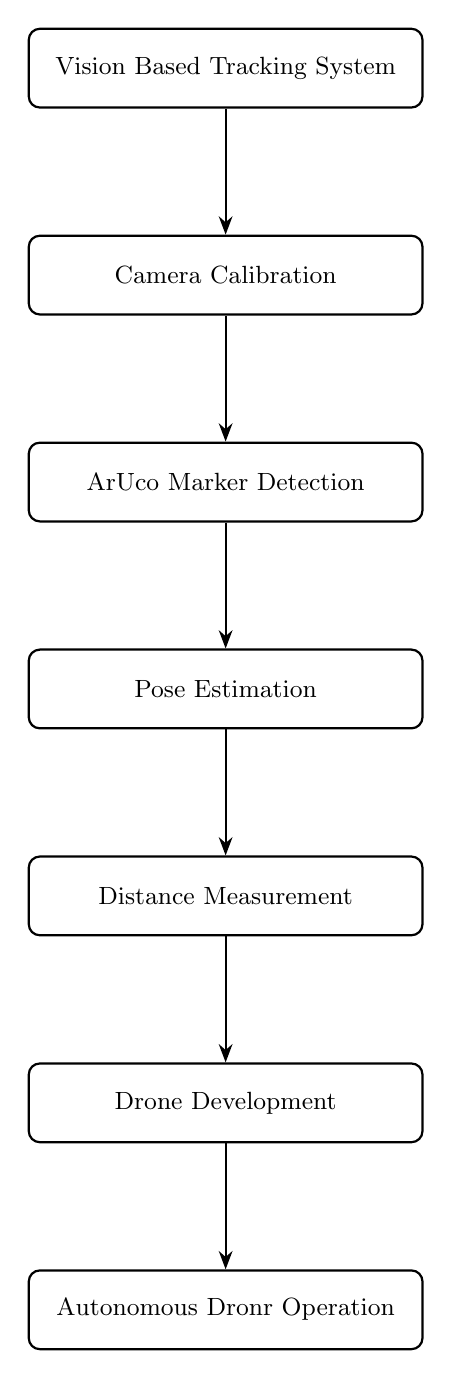
\begin{tikzpicture}[
node distance=1.6cm,
every node/.style={
draw,
rounded corners,
minimum width=5cm,
minimum height=1cm,
align=center,
font=\small
},
>=Stealth,
thick
]
\node (A) {Vision Based Tracking System};
\node (B) [below=of A] {Camera Calibration};
\node (C) [below=of B] {ArUco Marker Detection};
\node (D) [below=of C] {Pose Estimation};
\node (E) [below=of D] {Distance Measurement};
\node (F) [below=of E] {Drone Development};
\node (G) [below=of F] {Autonomous Dronr Operation};
\draw[->] (A)--(B);
\draw[->] (B)--(C);
\draw[->] (C)--(D);
\draw[->] (D)--(E);
\draw[->] (E)--(F);
\draw[->] (F)--(G);
\end{tikzpicture}
\caption{Overall workflow of the vision-based Autonomous Drone tracking system.}
\end{figure}
\newpage
\section{Tracking System Architecture}
The tracking system is built around a two-axis pan-tilt mechanism designed to provide independent rotational motion along the horizontal (X-axis) and vertical (Y-axis) directions. The assembly consists of two servo motors mounted on a custom-designed 3D-printed structure as shown in (Figure~\ref{fig:System Architecture}), which serves as a lightweight and rigid platform for the vision system.

The first servo motor is responsible for the pan motion, enabling the camera to rotate horizontally and track the target along the X-axis. The second servo motor is mounted on top of the pan mechanism and provides tilt motion, allowing the camera to rotate vertically along the Y-axis. This arrangement enables the camera to orient itself towards the target in both directions while maintaining smooth and controlled movement.

\begin{figure}[H]
\centering
\includegraphics[width=0.40\textwidth]{/home/lakshya/Downloads/system_architecture.jpeg}
\caption{System Architecture}
\label{fig:System Architecture}
\end{figure}

The entire pan-tilt assembly is fabricated using 3D-printed components specifically designed to ensure structural stability, accurate alignment of the servo motors, and sufficient mechanical freedom of movement. The lightweight construction minimizes the load on the servo motors while maintaining adequate rigidity, resulting in improved responsiveness and tracking accuracy.

A camera is securely mounted on the tilt platform, allowing it to capture real-time video frames. These images are processed using computer vision algorithms to determine the position of the target within the camera frame. The positional error between the target and the image center is then processed by a PID controller, which generates appropriate control signals for the servo motors. Consequently, the pan and tilt servos continuously adjust the camera orientation, ensuring that the target remains centered within the field of view.

The modular design of the tracking system also facilitates future integration with the autonomous drone platform, where the vision-based tracking algorithm can be extended from the stationary pan-tilt mechanism to active UAV navigation and target-following applications.
\subsection{Working Principle}
The working principle (Figure~\ref{fig:Workflow})of the tracking system is based on real-time visual feedback and closed-loop control. A camera mounted on the tilt platform continuously captures video frames of the surrounding environment. These frames are processed using computer vision algorithFigure~ms to detect and locate the target within the image.

Once the target is identified, its position is compared with the center of the image frame to determine the positional error along both the horizontal and vertical axes. This error represents how far the target is from the desired central position in the camera’s field of view.

The calculated error is then fed into a PID (Proportional–Integral–Derivative) controller, which computes the appropriate control signals required to minimize the error. Based on these signals, the pan and tilt servo motors are actuated to adjust the orientation of the camera accordingly.
\begin{figure}[H]
\centering

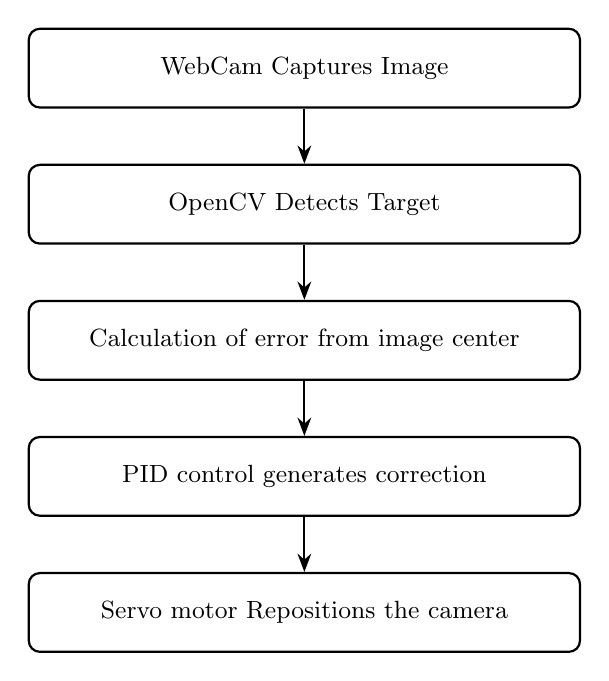
\begin{tikzpicture}[
node distance=0.7cm,
every node/.style={
draw,
rounded corners,
minimum width=7cm,
minimum height=1cm,
align=center,
font=\small
},
>=Stealth,
thick
]
\node (A) {WebCam Captures Image};
\node (B) [below=of A] {OpenCV Detects Target};
\node (C) [below=of B] {Calculation of error from image center};
\node (D) [below=of C] {PID control generates correction};
\node (E) [below=of D] {Servo motor Repositions the camera};
\draw[->] (A)--(B);
\draw[->] (B)--(C);
\draw[->] (C)--(D);
\draw[->] (D)--(E);
\end{tikzpicture}
\caption{Overall workflow of the tracking system.}
\label{fig:Workflow}
\end{figure}

\newpage
\subsection{PID Controls}
A Proportional–Integral–Derivative (PID) controller is one of the most widely used closed-loop feedback control algorithms in industrial automation and robotics. It continuously computes the error between a desired reference value (setpoint) and the measured process variable, and generates an appropriate control signal to minimize this error. In the present project, the PID controller is employed to regulate the motion of the pan and tilt servo motors, enabling the camera to continuously track an object and maintain it at the center of the camera frame.

The vision system determines the position of the target within each captured image frame. Any deviation of the target from the image center is treated as an error. Based on this error, the PID controller computes the required correction in the servo angles so that the camera smoothly follows the target
\subsubsection{Error Calculation}
Let

\[x_c = \text{be the horizontal center of camera frame}\]
\[y_c = \text{be the vertical center of the camera frame}\]
\[x_t = \text{be the detected horizontal coordinate of the target}\]
\[y_t = \text{be the detected vertical coordinate of the target.}\]
Tracking errors are defined as:
\begin{equation}
e_x(t)=x_c-x_t
\end{equation}
and
\begin{equation}
e_y(t)=y_c-y_t
\end{equation}
where,
\[e_x(t) \text{ represent horizontal tracking error}\]
\[e_y(t) \text{ represents vertical tracking erro}\] \\

The objective of the controller is to minimize both errors so that the target remains centered within the camera's field of view.
\newpage
\paragraph{Proportional Control:}
The proportional component generates a correction proportional to the instantaneous tracking error,
\begin{equation}
P(t)=K_Pe(t)
\label{eq:proportional}
\end{equation}
A larger positional error results in a larger corrective motion of the servo. \textbf{Increasing $K_P$ improves the response speed}; however, excessively large values may introduce oscillations and overshoot.
\paragraph{Integral Control:}
The integral component accumulates the tracking error over time,
\begin{equation}
I(t) =K_I\int e(t)\,dt
\label{eq:integral}
\end{equation}
Its primary function is to \textbf{eliminate steady-state error}. If the target remains slightly displaced from the image center for an extended period, the integral term gradually increases the corrective action until the error becomes zero.
\paragraph{Derivative Control:}
The derivative component predicts the future behaviour of the error by considering its rate of change,
\begin{equation}
D(t) = K_D\frac{de(t)}{dt}
\label{eq:derivative}
\end{equation}
This term provides damping to the system and \textbf{reduces oscillations}. It enables smoother camera motion by slowing the servo movement as the target approaches the image center.

The output of PID control is given by:
\begin{equation}
u(t) = P(t) + I(t) + D(t)
\label{eq:PID}
\end{equation}
from eq(\ref{eq:proportional}), eq(\ref{eq:integral}) and eq(\ref{eq:derivative}) we have.
\begin{equation}
u(t)=K_Pe(t)+K_I\int e(t)\,dt
+K_D\frac{de(t)}{dt}
\label{eq:complete PID}
\end{equation}
where,
\vspace{0.5cm}
\newline
$u(t) = $ is the control signal,\\
$e(t) = $ is the tracking error,\\
$K_P = $ is the proportional gain,\\
$K_I = $ is the integral gain,\\
$K_D = $ is the derivative gain.

The controller output is applied to the servo motor, which adjusts the camera orientation.
\newpage
\begin{figure}
\centering
\includegraphics[width=18cm,height=7cm]{/home/lakshya/Downloads/Cohen-Coon-diagram.jpg}
\caption{PID Curve.}
\label{fig:PID curve}
\end{figure}
\subsection{Challanges Encountered and Solutions}

\begin{enumerate}[label=\roman*.]
\item{\textbf{Camera latency} : the time delay between an event occurring in the real world and the image data being available to the processing system.}
\subsubsection*{Solution:}
\begin{itemize}
\item{Lower the camera resolution (ex: 640×480 instead of 1920×1080)}
\item{Increase the camera frame rate (30–60 FPS)}
\item{Use a faster camera interface (CSI camera instead of USB)}
\item{Reduce image buffering by always processing the latest frame.}
\end{itemize}
\item{\textbf{Servo jitter} : rapid, unwanted oscillations of the motor when it is supposed to be holding a steady position.}
\subsubsection*{Solution:}
\begin{itemize}
\item{Tune PID gains properly (\textbf{reduce Kp if oscillating}).}
\item{\textbf{Reduce Kd }if derivative noise causes vibration}
\item{Introduce a dead zone (ex: ±10–20 pixels around the image center).}
\item{Use a stable power supply dedicated to the servo.}
\item{Minimize mechanical backlash by tightening the servo mount.}
\end{itemize}
\item{\textbf{Tracking Instability} : the overall failure of the system to maintain a lock on the target, or sustained oscillations}
\subsubsection*{Solution:}
\begin{itemize}
\item{Improve camera calibration to reduce pose estimation errors.}
\item{Tune the PID controller correctly.}
\item{Increase camera frame rate.}
\item{Prevent the servo from operating near its mechanical limits.}
\item{Secure the camera and servo mount to minimize vibrations.}

\end{itemize}
\item{\textbf{Lightening Sensitivity} : describes how dependent the tracking algorithm is on consistent illumination to detect the target.}
\subsubsection*{Solution:}
\begin{itemize}
\item{Maintain consistent indoor lighting.}
\item{Disable automatic exposure and white balance if the camera allows it.}
\item{Use high-contrast ArUco markers printed on matte paper.}
\item{Reduce reflections and shadows around the target.}
\end{itemize}
\item{\textbf{PID Tuning} : the process of calibrating the three control parameters-Proportional (P), Integral (I), and Derivative (D) to ensure the servo responds accurately to errors.}
\end{enumerate}
\newpage
\section{Camera Calibration}
\begin{figure}[H]
\centering
\includegraphics[width=8.0cm=\textwidth]{/home/lakshya/Downloads/corners_calib_4.jpg}
\caption{Chessboard Based  Camera Calibration.}
\label{fig:chessboard}
\end{figure}

Camera calibration (need help? = \href{https://github.com/Mark42-Lakshya/Fly_High/blob/main/README.md}{visit here}) is the process of estimating the parameters of a camera's lens and image sensor. These parameters can be used to correct for lens distortion, measure the size of an object in world units, or determine the location of the camera in the scene.\\

This toolkit includes:
\begin{enumerate}[label=\roman*.]
\item{\textbf{Image Capture Tool}: Capture calibration images from your camera.}
\item{\textbf{Calibration Tool}: Process the calibration images to compute camera parameters.}
%\item{\textbf{Live Undistortion}: Apply the calibration to a live video feed}
\end{enumerate}
\large{\textbf{Requirement}:}
Python 3.6+, 
OpenCV 4.5+, 
NumPy 1.20+
\newpage
\subsection{Calibration Results}
\thispagestyle{introstyle}
\begin{enumerate}[label=\roman*.]
\item{\textbf{intrinsic camera matrix}: defines how the camera projects 3D points onto the 2D image plane. it's a $3\times{3}$ matrix estimated during calibration.}
\item{$f_x$ and $f_y$ are focal lenghts in pixel units.}
\item{$C_x$ and $C_y$ are the optical center near the image cente.}
\item{\textbf{Distortion Coefficient}: Real lense introduce geometric distortion that deviate from the ideal pinhole model.}
\end{enumerate}

\[
K = \begin{pmatrix}
f_x & 0 & C_x \\
0 & f_y & C_y \\
0 & 0 & 1
\end{pmatrix}
\]
\vspace{0.5cm}
\begin{table}[H]
\centering
\caption{Calibration Quality Based on Reprojection Error}
\label{tab:reprojection_error}
\begin{tabular}{cc}
\toprule
\textbf{Reprojection Error (pixels)} & \textbf{Calibration Quality} \\
\midrule
$<0.3$ & Excellent \\
$0.3-0.5$ & Very Good \\
$0.5-1.0$ & Acceptable \\
$>1.0$ & Calibration should be improved \\
\bottomrule
\end{tabular}
\end{table}
\newpage
\section{ArUco Marker/April Tag Detection}
\textbf{ArUco markers} are binary square fiducial marker designed for fast detection and pose estimation in computer vision applications.
\begin{figure}[H]
\centering
\includegraphics[width=10.0cm=\textwidth]{/home/lakshya/Downloads/marker_detection.png}
\caption{Aruco Marker ID:23}
\label{fig:aruco marker}
\end{figure}
\subsection{Pose and Distance Estimation}
Pose estimation is the process of determining the position and orientation of an object relative to the camera or another reference frame.

In the context of ArUco markers, pose estimation computes the 6 Degrees of Freedom (6-DoF) of the marker using the camera's intrinsic parameters and the known physical size of the marker.\\
The six degrees of freedom are:
\begin{enumerate}[label=\roman*.]
\item{Position (Translation):
\begin{itemize}
\item{\textbf{x}: Left-Right Displacement}
\item{\textbf{y}: Up-Down displacement}
\item{\textbf{z}: Distance from the camera}
\end{itemize}
}
\item{Orientation (Rotation):
\begin{itemize}
\item{\textbf{Roll}: Rotation about the X-axis}
\item{\textbf{Pitch}: Rotation about y-axis}
\item{\textbf{Yaw}: Rotation about the z-axis}
\end{itemize}}
\end{enumerate}
\newpage
\thispagestyle{introstyle}
The pose estimation is represented by:

\large{\textbf{Translation Vector}:}
\[
t = \begin{bmatrix}
t_x \\
t_y \\
t_z
\end{bmatrix}
\]
where,

\[t_x = \text{Horizontal position}\]
\[t_y = \text{Vertical position}\]
\[t_z = \text{Distance from the camera}
\]

\large{\textbf{Rotation Vector}:}
\[
r = \begin{bmatrix}
r_x \\
r_y \\
r_z
\end{bmatrix}
\]
where,

\[r_x = \text{x-component of rotation vector}\]
\[r_y = \text{y-component of rotation vector}\]
\[r_z = \text{z-component of rotation vector}\]

Also, \textbf{$t_z$} is the actual distance of the marker from the camera.
\newpage
\section{Transition to Drone Platform}
\begin{figure}[H]
\centering
\includegraphics[width=7.9cm=\textwidth]{/home/lakshya/Downloads/drone.jpeg}
\caption{Drone}
\label{fig:drone}
\end{figure}
\subsection{Development Process}

\begin{figure}[H]
\centering

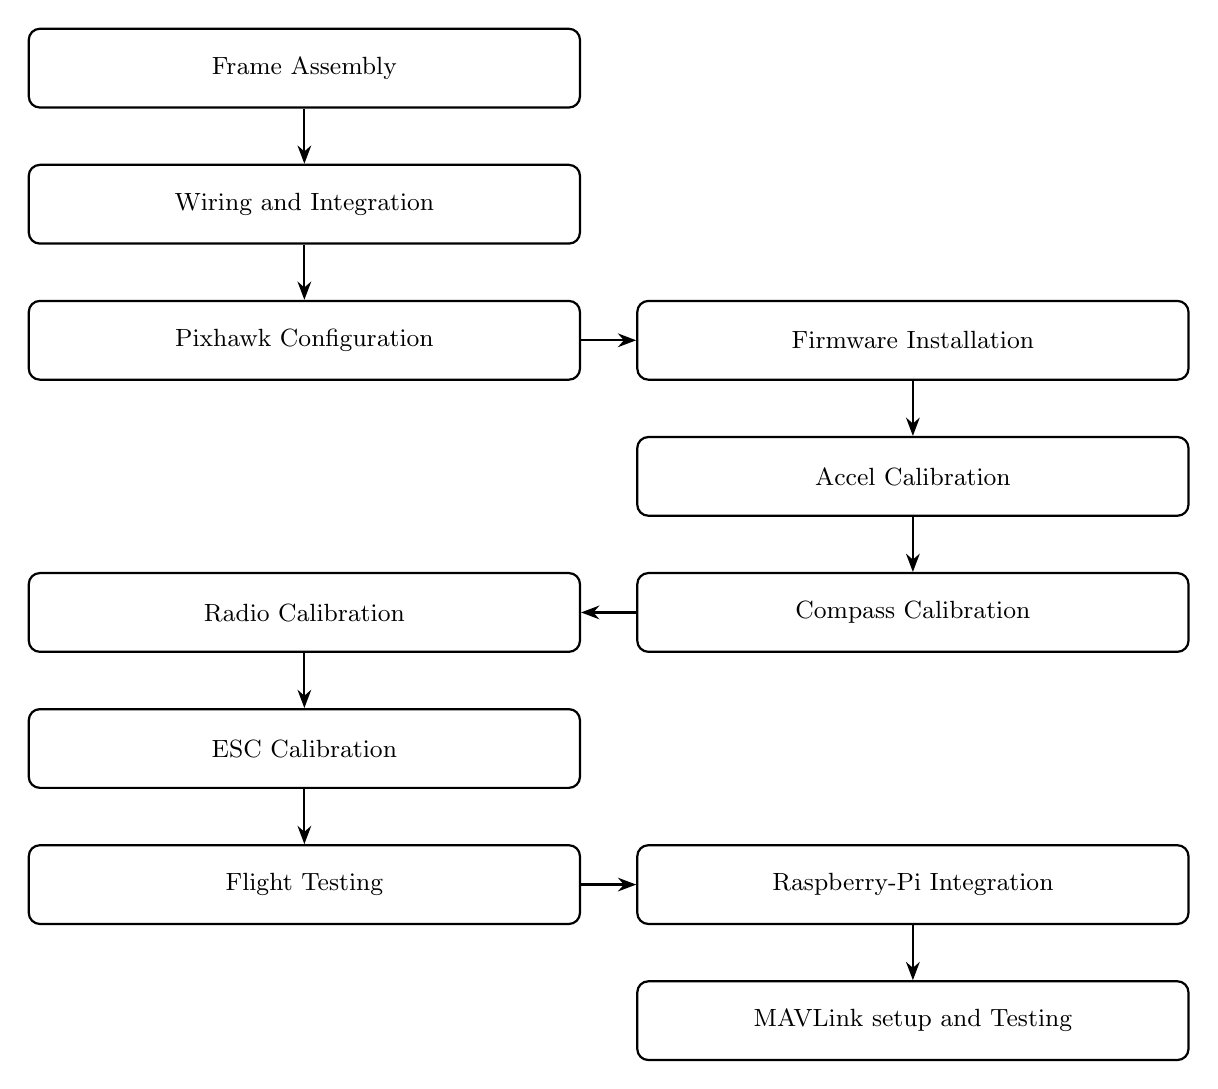
\begin{tikzpicture}[
node distance=0.7cm,
every node/.style={
draw,
rounded corners,
minimum width=7cm,
minimum height=1cm,
align=center,
font=\small
},
>=Stealth,
thick
]
\node (A) {Frame Assembly};
\node (B) [below=of A] {Wiring and Integration};
\node (C) [below=of B] {Pixhawk Configuration};
\node (D) [right=of C] {Firmware Installation};
\node (E) [below=of D] {Accel Calibration};
\node (F) [below=of E] {Compass Calibration};
\node (G) [left=of F] {Radio Calibration};
\node (H) [below=of G] {ESC Calibration};
\node (I) [below=of H] {Flight Testing};
\node (J) [right=of I] {Raspberry-Pi Integration};
\node (K) [below=of J] {MAVLink setup and Testing};
\draw[->] (A)--(B);
\draw[->] (B)--(C);
\draw[->] (C)--(D);
\draw[->] (D)--(E);
\draw[->] (E)--(F);
\draw[->] (F)--(G);
\draw[->] (G)--(H);
\draw[->] (H)--(I);
\draw[->] (I)--(J);
\draw[->] (J)--(K);
\end{tikzpicture}
\caption{Overall workflow for Drone Development.}
\label{fig:workflow2}
\end{figure}
\newpage
\subsubsection{System Architecture and Making}

The quadcopter was designed by integrating the mechanical frame, propulsion system, flight controller, power distribution system, and communication modules into a single aerial platform. The primary objective was to develop a stable drone capable of autonomous flight while allowing future integration with computer vision algorithms.

The drone consists of four brushless DC motors mounted on a quadcopter frame in an X-configuration. Each motor is controlled by a dedicated Electronic Speed Controller (ESC), which receives PWM signals from the Pixhawk flight controller. A Lithium Polymer (Li-Po) battery supplies power to the entire system through a Power Distribution Board (PDB), ensuring uniform power delivery to all ESCs and onboard electronics.

The Pixhawk 2.4.8 flight controller acts as the central processing unit of the drone. It acquires data from onboard sensors such as the Inertial Measurement Unit (IMU), barometer, magnetometer, and GPS receiver. Using these measurements, the controller estimates the attitude and position of the drone and generates appropriate motor commands to maintain stable flight.

A Raspberry Pi 4 serves as the companion computer. It is connected to the Pixhawk through the MAVLink communication protocol via the TELEM2 serial interface. The Raspberry Pi executes high-level tasks such as computer vision, object detection, autonomous navigation, and mission planning, while Pixhawk handles the low-level flight stabilization.

The Ground Control Station (Mission Planner) communicates with the Pixhawk through telemetry or MAVLink-over-UDP, allowing real-time monitoring, parameter tuning, calibration, and autonomous mission execution.
\newpage
\subsubsection{Programming and calibration}
Before flight operations, all sensors and communication interfaces must be calibrated to ensure accurate state estimation and reliable flight performance. Mission Planner (\textbf{mission planner programing guid:} \href{https://github.com/Mark42-Lakshya/Fly_High/blob/main/mission_planner_guid.txt}{visit}) software was used to configure the Pixhawk flight controller and perform all necessary calibration procedures.

\paragraph{Compass Calibration:}
The compass (magnetometer) provides heading information by measuring the Earth's magnetic field. Accurate heading estimation is essential for waypoint navigation, position hold, return-to-launch (\textbf{RTL}), and autonomous flight.
During calibration, \textbf{the drone was rotated through all orientations }until sufficient magnetic field samples were collected. Mission Planner computed the magnetic offsets for each axis to compensate for hard-iron and soft-iron distortions caused by nearby electronic components.
\begin{figure}[H]
\centering
\includegraphics[width=10.0cm=\textwidth]{/home/lakshya/Downloads/compass_calibration.png}
\caption{Compass Calibration.}
\label{fig:compass calibration}
\end{figure}
\textbf{Why proper compasss calibration is needed?}
\begin{enumerate}[label=\roman*.]
\item{Accurate yaw estimation}
\item{Improved GPS navigation}
\item{Stable Loiter mode}
\item{Reliable Return-to-Launch functionality}
\end{enumerate}
\Large{\textbf{Note:}}
Avoid calibrating inside the closed room or area, also keep distance from heavy electronic devices while calibrating! 
\newpage
\paragraph{Accelerometer calibration:}
The accelerometer measures linear acceleration along the three body axes.
The Pixhawk requires calibration to determine the sensor bias and scale factors. \\ \textbf{During calibration, the drone was placed in six different known orientations}:
\begin{figure}[H]
\centering
\includegraphics[width=10.0cm=\textwidth]{/home/lakshya/Downloads/accelerometer_calibration.png}
\caption{Accelerometer Calibration.}
\label{fig:accelerometer calibration}
\end{figure}
\begin{enumerate}[label=\roman*.]
\item{Level}
\item{Left Side}
\item{Right Side}
\item{Nose Up}
\item{Nose Down}
\item{Upside Down}
\end{enumerate}

These measurements allow the Pixhawk to estimate sensor offsets. Proper accelerometer calibration improves:\\
\textbf{A}ttitude estimation,
\textbf{S}table hovering,
\textbf{S}mooth takeoff,
\textbf{A}ccurate position control.\\
\Large{\textbf{Note:}} Poor calibration causes the drone to drift, lean during takeoff, or exhibit unstable hovering behavior.

\newpage
\paragraph{Radio Calibration:}
Radio calibration establishes the relationship between transmitter stick positions and the PWM values received by the Pixhawk.The transmitter sticks were moved through their complete range while Mission Planner recorded
minimum PWM,
maximum PWM,
trim value,
channel direction.

\begin{figure}[H]
\centering
\includegraphics[width=10.0cm=\textwidth]{/home/lakshya/Downloads/radio_calibration.jpg}
\caption{Radio Calibration.}
\label{fig:Radio calibration}
\end{figure}

\begin{figure}[H]
\centering
\includegraphics[width=10.0cm=\textwidth]{/home/lakshya/Downloads/mp_radio_calib.jpg}
\caption{Mission Planner Interface.}
\label{fig:Radio calibration}
\end{figure}
\newpage
\paragraph{ESC Calibration}
Electronic Speed Controllers convert PWM signals from the Pixhawk into three-phase voltages for driving the brushless motors.ESC calibration synchronizes the throttle range between the Pixhawk and all ESCs.\\
During calibration:
\begin{enumerate}[label=\roman*.]
\item{Maximum throttle signal is transmitted,}
\item{Battery is connected,}
\item{Minimum throttle signal is sent.}
\end{enumerate}
The ESC stores these limits internally.Proper calibration ensures:
\begin{enumerate}[label=\roman*.]
\item{Simultaneous motor startup,}
\item{Equal thrust generation,}
\item{Smoother flight,}
\item{Better altitude stability.}
\end{enumerate}
Without calibration, motors may start at different throttle values, producing asymmetric thrust and unstable flight.\\

\begin{figure}[H]
\begin{minipage}{0.30\textwidth}
%\vspace{0.08cm}\\
\begin{figure}[H]
\centering

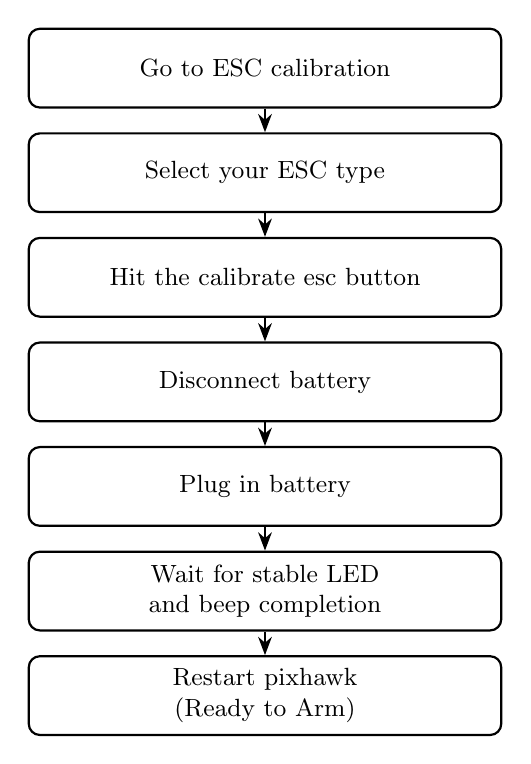
\begin{tikzpicture}[
node distance=0.3cm,
every node/.style={
draw,
rounded corners,
minimum width=6cm,
minimum height=1cm,
align=center,
font=\small
},
>=Stealth,
thick
]
\node (A) {Go to ESC calibration};
\node (B) [below=of A] {Select your ESC type};
\node (C) [below=of B] {Hit the calibrate esc button};
\node (D) [below=of C] {Disconnect battery};
\node (E) [below=of D] {Plug in battery};
\node (F) [below=of E] {Wait for stable LED \\and beep completion};
\node (G) [below=of F] {Restart pixhawk \\(Ready to Arm)};
\draw[->] (A)--(B);
\draw[->] (B)--(C);
\draw[->] (C)--(D);
\draw[->] (D)--(E);
\draw[->] (E)--(F);
\draw[->] (F)--(G);
\end{tikzpicture}
\label{fig:workflow}
\end{figure}
\end{minipage}
\hfill
\begin{minipage}{0.6\textwidth}
\centering
\includegraphics[width=12.0cm=\linewidth]{/home/lakshya/Downloads/mp_esc_config.jpeg}
\caption{Mission Planner Interface.}
\label{fig:mp interface}
\end{minipage}
\end{figure}
\newpage
\subsubsection{Flight Modes setup}
Different flight modes were configured using Mission Planner according to the requirements of the project.
\subsection*{Stabilize Mode:}The pilot controls the drone manually while Pixhawk stabilizes the roll, pitch, and yaw angles using the IMU measurements.
\subsection*{AltHold Mode:}The flight controller automatically maintains altitude using the onboard barometer while allowing manual horizontal movement.
\subsection*{Loiter Mode:}The drone maintains both its position and altitude using GPS, compass, barometer, and IMU data. This mode was primarily used for stable hovering during testing.
\subsection*{Guided Mode:}Guided mode allows external computers such as the Raspberry Pi to control the drone using MAVLink commands. This mode is essential for autonomous navigation and computer vision-based applications.
\subsection*{Return-to-Launch (RTL):}If communication is lost or RTL is manually activated, the drone automatically returns to the takeoff location using GPS navigation before landing safely.
\newpage
\subsection{Flight Testing}
After completing the mechanical assembly and sensor calibration, several flight tests were conducted to verify the stability and reliability of the drone.\\
\Large{\textbf{Note: }}For arming, Down the Throttle and move it to extrem Left or Right. Same for disarming.
%\subsection{Challenges Encountered and Solutions}
\section{Setting-up MAVLink Protocol}
MAVLink (Micro Air Vehicle Link) is a lightweight communication protocol used for exchanging telemetry, commands, and sensor data between the flight controller, companion computer, and Ground Control Station.
Our project uses MAVLink to establish communication between the Pixhawk flight controller, Raspberry Pi companion computer, and Mission Planner.
\subsection{Process}
\subsubsection{Raspberry-Pi Installation and setup}
The Raspberry Pi 4 Model B was configured with Raspberry Pi OS and connected to the local wireless network (\textbf{Raspberry-Pi setup guid:} \href{https://github.com/Mark42-Lakshya/Fly_High/blob/main/Raspberry_pi_setup_guid.md}{here}). Python packages required for MAVLink communication, including \textbf{pymavlink} and \textbf{MAVProxy}, were installed. \textbf{SSH} was enabled to allow remote access from a laptop, simplifying software development and debugging.
\subsubsection{Connecting pixhawk to Rpi through MAVLink}
Before proceeding further make sure that \textbf{Rpi and your computer should connected to the same network}. Open terminal in your computer device and do as follows:
\begin{enumerate}[label=\roman*.]
\item{Login to your companion computer (\textbf{here it is our Rpi}): Type, \textbf{ssh} \verb|<host_name>@<network_IP_on_Rpi>|}
\begin{figure}[H]
\centering
\includegraphics[width=\textwidth]{/home/lakshya/Downloads/login.png}
\label{fig:ssh login}
\end{figure}
\item{Login to Drone \textbf{Virtual environment}: Locate your environment directory, \\\textbf{for example}: Type:  \verb|source ~/drone_env/bin/activate|}
\item{Build UDP connection with mission planner: for example: Type:\\  \verb|mavproxy.py   --master=/dev/serial0   --baudrate 57600|\\   \verb|--out=udp:<PC_IP>:14550|}
\item{Now, after this whole configuration you can able to see your flight data in your laptop or pc terminal wirelessly.}
\end{enumerate}
\section{Performing Autonomous Actions}
Now, we can give python commands to rpi to perform autonomous actions. \textbf{For example:} here is a sample code that can arm the drone and takeoff to 1 meter height and hover for 30 seconds and land.\\ 
\begin{lstlisting}[caption={Simple Python Program},label={lst:python}]
from pymavlink import mavutil
import time
# master = mavutil.mavlink_connection('/dev/ttyAMA0', baud=57600)
master = mavutil.mavlink_connection('udp:127.0.0.1:14551') # Mission planner uses 14550 and rpi uses 14551 that's why
# allow us to run MP at the same time.
print("Waiting for heartbeat...")
master.wait_heartbeat()
print("Connected!")
# GUIDED mode
mode = master.mode_mapping()['GUIDED']
master.mav.set_mode_send(
    master.target_system,
    mavutil.mavlink.MAV_MODE_FLAG_CUSTOM_MODE_ENABLED,
    mode)
print()

# Check current mode
while True:
    msg = master.recv_match(type='HEARTBEAT', blocking=True)
    print("Mode:", mavutil.mode_string_v10(msg))
    current_mode = mavutil.mode_string_v10(msg)
    print("Current Mode:", current_mode)
    if current_mode == "GUIDED":
        print("GUIDED mode confirmed")
        break
time.sleep(2)
# Arm
master.arducopter_arm()
master.motors_armed_wait()
print("Armed!")
# Takeoff to 1 meter
master.mav.command_long_send(
    master.target_system,
    master.target_component,
    mavutil.mavlink.MAV_CMD_NAV_TAKEOFF,
    0,
    0, 0, 0, 0,
    0, 0,
    1.0)
print("Taking off...")
# Monitor altitude
while True:
    msg = master.recv_match(type='GLOBAL_POSITION_INT', blocking=True)
    alt = msg.relative_alt / 1000.0  # mm -> m
    print(f"Altitude: {alt:.2f} m")
    if alt >= 0.95:
        print("Reached target altitude")
        break
print("Hovering for 30 seconds...")
time.sleep(30)
print("Landing...")
master.mav.command_long_send(
    master.target_system,
    master.target_component,
    mavutil.mavlink.MAV_CMD_NAV_LAND,
    0,
    0, 0, 0, 0,
    0, 0, 0)
while True:
    msg = master.recv_match(type='GLOBAL_POSITION_INT', blocking=True)
    alt = msg.relative_alt / 1000.0
    print(f"Altitude: {alt:.2f} m")
    if alt <= 0.1:
        print("Landed")
        break
\end{lstlisting}
\thispagestyle{introstyle}
\end{document}
